\section{Introduction}
\label{sec:introduction}

A distributed ledger (DL) is a database that tolerates nodes with malicious intentions in a distributed manner.
And distributed ledger technology (DLT) enables the realization and operation of distributed ledgers,
which allows almost all the nodes in the network, to agree on an almost immutable record of transactions with Byzantine failure tolerance (BFT) and eventual consistency via a predefined consensus mechanism \cite{Sunyaev2020}.
Blockchain is one of the most well-known DLTs which was first implemented on Bitcoin. It proposed a simple but robust way for transaction data storage without relying on the trust of third parties \cite{nakamoto2008peer}.
Blockchain also ensures improved security and anonymity of Bitcoin transactions compared with traditional electronic transactions.
Since the introduction of Bitcoin in 2009, DLT based cryptocurrencies have made a great impact on financial industries. After this people also discovered that the usefulness of DLTs is beyond the exchange of currencies and
significant adoption of DLTs was made in many other industries for other different services.
Namecoin is the first altcoin\footnote{Altcoin: any cryptocurrencies that are not Bitcoin.} for being the first to create its own blockchain separate from Bitcoin's \cite{kalodner2015empirical}.
And its functionalities are not limited to financial transactions.
The creation of Namecoin was inspired by the idea of BitDNS \cite{merited2010bitdns} and for establishing a decentralized domain name looking-up system.


The Internet today is a widespread information infrastructure and its history can date back to the 1970s when ARPANET\footnote{ARPANET: Advanced Research Projects Agency Network.
    The first wide-area packet-switching network with distributed control originally established by the United States Department of Defense.} was developed.
For most of the current Internet applications, data is stored in a centralized manner and users do not own data by themselves. As shown in Fig~\ref{fig:traditional_internet},
if users want to do actions like checking their emails or browsing the content of a website, first, they need to connect to the web servers via the Internet with web browsers, then the web servers retrieve the data from the database and then send it back to users.
Usually, users' data is hidden behind service providers' application code. This kind of arrangement has been very successful as it is easy to implement. However, it is not ideal since:
\begin{itemize}
    \item Users must use the requested web user interface if they want to access their data.
    \item The websites control the rules and access rights of the data.
    \item The websites may snoop your data and sell users' information to others.
    \item Illegal use of data by websites' employees for personal purposes.
\end{itemize}

\begin{figure}[h]
    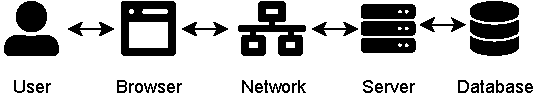
\includegraphics[width=0.45\textwidth,trim={-1cm 0 0.25cm 0},clip]{figs/traditional_internet.pdf}
    \caption{User data arrangement of traditional (centralized) Internet application}
    \label{fig:traditional_internet}
\end{figure}

Since the early Internet, hosts in the network were assigned names for more convenient use and memorization by humans. With the growth of the network, it became impossible to store all the hosts in a single table.
And Domain Name System (DNS) invented by Paul Mockapetris of USC/ISI permitted a scalable distributed mechanism for resolving hierarchical host names into Internet addresses \cite{leiner2009brief}.
Now the coordination and management of DNS Root, IP Addressing, and other Internet protocols are in the charge of IANA\footnote{IANA: Internet Assigned Numbers Authority. Website: \url{https://www.iana.org}} \cite{Postel1994DomainNS}.
These DNS root servers are central nodes of trust and failure, and cyber-attack such as DDoS\footnote{DDoS: Distributed Denial-of-service Attack.
    Usually, the attack attempts to disrupt the normal traffic of the victim's server by a large number of requests made by attacker devices.} towards them may lead to the whole system taken down.
It is reported that a large-scale DDoS attack was launched towards 13 root servers on March 21st, 2002. Fortunately, the attack only lasted for one hour and didn't cause severe damage \cite{mcguire2002attack}.
Besides, these central points may also be exploited and misleading users into connecting to malicious websites like the Turkish fake site certs incident \cite{rosenblatt_2013}.


Internet-of-Things (IoT) refers to \textit{``physical or virtual objects which connect to the Internet and has the ability to communicate with human users or other objects"} \cite{6978614}.
These devices such as smart webcam and wearable health monitors are widely used in our daily life.
It is estimated that there will be approximately 30.9 billion active IoT device connections installed worldwide by 2021 \cite{statista_2021}.
Due to the heterogeneity and complexity of IoT devices, their security and privacy issues are becoming more and more severe \cite{6978614}.
With the increasing number of devices connected to the network, the load of centralized servers for handling the connection will become much higher.
DLT supported IoT has been created for addressing the challenges like security, data integrity, and reliability, and secured P2P sharing.
It is a new decentralized and distributed solution to IoT services and enables the opportunity for developing new and creative applications and business models in vertical domains, e.g., from healthcare to supply chain, energy industry, and smart manufacturing \cite{Farahani2020TheCO}.


\begin{onehalfspace}
\end{onehalfspace}
\noindent\textbf{Motivation.} Many data management issues related to security, integrity, access control have been exposed from the centralized data model of the traditional Internet.
When accessing web services, user data control is maintained by service vendors rather than users themselves.
Domain Name System containing central nodes like DNS root servers are vulnerable to cyber attacks such as DDoS.
We wish to re-decentralize the current Internet service via distributed ledger technology for better security and data integrity.
Distributed ledger technologies like blockchain enhance the security and data integrity of IoT services.
However, many current DLTs are based on Proof-of-Work (PoW) consensus mechanism \cite{10.1145/2976749.2978341}, requesting strong computing power and huge energy consumption for solving hash computational puzzles.
These mechanisms are not suitable for IoT devices that have limited computational power and energy consumption restriction. In addition, transaction fees paid to the miners in the network caused an extra cost for the service.
DLTs like Bitcoin blockchain are also facing problems like low TPS\footnote{TPS: Transaction Per Second. The approximate average TPS of Bitcoin blockchain is around 5.}, bad scalability, etc.
They are not suitable for IoT service scenarios like sending a large number of micro-transactions in a short period of time. 
In summary, we want to use a feeless, lightweight, and scalable DLT that can support IoT use cases.


\begin{onehalfspace}
\end{onehalfspace}
\noindent\textbf{Contribution.} We introduce the design of Vivian, a decentralized global naming and storage system secured by IOTA Tangle distributed ledger \cite{popov2015tangle}.
It is a new decentralized Public Key Infrastructure (PKI) system that enables users to register human-readable and unique domain names with the binding information.
In the system, there are no central trust points and users control their own data.
We describe the structure of the system: Tangle DL layer, peer network layer, and storage layer.
Tangle distributed ledger layer records critical data bindings. Peer network layer handles user queries and helps users find the binding value of the names quickly.
Storage layer stores user data under users' control securely and the storage providers cannot tamper with the data.
We describe the implementation of Tangle DL for critical data binding and naming operations.
We also describe the P2P network implementation including peer discovery and peer communication.
In addition, we evaluate the system's compatibility on IoT devices and discuss the application of the system in real-world scenarios.